\documentclass[a4paper,12pt]{article}

\usepackage{graphicx}  % For including images
\usepackage{listings}  % For code formatting
\usepackage{xcolor}    % For color in code
%\usepackage{hyperref}  % For clickable links
\usepackage[T1]{fontenc} 

\usepackage{amsmath}
\usepackage{subcaption}
\usepackage{float} % Add this in your preamble
\usepackage[colorlinks=true, linkcolor=black, urlcolor=blue, citecolor=blue]{hyperref}

% Define Python code style
\lstdefinestyle{python}{
    language=Python,
    basicstyle=\ttfamily\small,
    keywordstyle=\color{blue},
    commentstyle=\color{gray},
    stringstyle=\color{red},
    numbers=left,
    numberstyle=\tiny,
    stepnumber=1,
    breaklines=true,
    frame=single,
    backgroundcolor=\color{lightgray!20}
}

\title{\textbf{Assignment 1 - Pattern Recognition (PMAT 403)}}
\author{\textbf{Gandholi Sarat - 23008 } }


\date{\today}

\begin{document}


\maketitle


\section*{Link to Notebook}
\href{https://colab.research.google.com/drive/1zJLuFBV0DYH311h503UJMq7Wiyi12hVe?usp=sharing}{Click here to access the Colab Notebook}

\tableofcontents
\listoffigures
\newpage


\section{Computer Programs}

\subsection{Question 1: Data Generator}
\textbf{Answer:} Generates a two-class, two-dimensional dataset using four normal distributions.  
The first two distributions belong to class +1, the last two belong to class -1.

\textbf{Parameters:}
\begin{itemize}
    \item \textbf{m:} 2x4 matrix, where each column is the mean vector for a distribution.
    \item \textbf{s:} Variance parameter.
    \item \textbf{N:} Number of points to generate per distribution.
    \item \textbf{seed:} Random seed for reproducibility (optional).
\end{itemize}

\textbf{Returns:}
\begin{itemize}
    \item \textbf{X:} 2x(4*N) data matrix.
    \item \textbf{y:} (4*N) class labels vector.
\end{itemize}
\begin{lstlisting}[style=python]
    import random
    import math

    if seed is not None:
        np.random.seed(seed)  # Ensure reproducibility
    X = []
    y = []
    S = s * np.eye(2)

    for i in range(4):
        mean = np.array(m)[:, i]
        samples = np.random.multivariate_normal(m[:, i], S, N).T
        X.append(samples)
        y.append(np.ones(N) if i < 2 else -np.ones(N))  
    X = np.concatenate(X,1)  # Shape: (2, 4N)
    y = np.concatenate(y)  # Shape: (4N,)

    return X.T, y  # Transpose X to have shape (4N, 2)
\end{lstlisting}
\newpage
\iffalse
\begin{figure}[h]
    \centering
    %\includegraphics[width=0.7\textwidth]{plot1.png}
    \caption{Graph of $y = x^2$}
    \label{fig:plot1}
\end{figure}
\fi

\subsection{Question 2: Neural network }
\textbf{Answer:} The network uses the tanh activation function and supports three training methods: standard backpropagation, backpropagation with momentum, and backpropagation with an adaptive learning rate.
The network is initialized with random weights and biases, and the training process includes forward propagation, loss calculation, and weight updates based on the chosen method.

\begin{lstlisting}[style=python]
    import numpy as np
    
    class NeuralNetwork:
        def __init__(self, input_dim, hidden_nodes):
            self.input_dim = input_dim
            self.hidden_nodes = hidden_nodes
            self.output_dim = 1  # Single output node
    
            # Initialize weights using uniform random values between -0.5 and 0.5
            self.W1 = np.random.uniform(-0.5, 0.5, (input_dim, hidden_nodes))  
            self.b1 = np.random.uniform(-0.5, 0.5, (1, hidden_nodes))  
            self.W2 = np.random.uniform(-0.5, 0.5, (hidden_nodes, 1))  
            self.b2 = np.random.uniform(-0.5, 0.5, (1, 1))  
    
        def tanh(self, x):
            #Tanh activation function: f(x) = (e^x - e^(-x)) / (e^x + e^(-x))
            return np.tanh(x)
    
        def tanh_derivative(self, x):
            #Derivative of tanh: f'(x) = 1 - tanh^2(x)
            return 1 - np.tanh(x) ** 2
    
        def forward(self, x):
            #Compute forward pass
            self.hidden_input = np.dot(x, self.W1) + self.b1
            self.hidden_output = self.tanh(self.hidden_input)
    
            self.final_input = np.dot(self.hidden_output, self.W2) + self.b2
            self.final_output = self.tanh(self.final_input)  
    
            return self.final_output
    
        def loss(self, y_true, y_pred):
            #Mean Squared Error Loss function
            return np.mean((y_true - y_pred) ** 2)
    
        def train(self, X, y, method, epochs, params):
            #Train the neural network using different optimization methods
            x = X.T
            lr, mc, lr_inc, lr_dec, max_perf_inc = params  # Unpack hyperparameters
    
            prev_loss = float('inf')  # Initialize previous loss for adaptive learning rate
    
            # Initialize momentum variables
            velocity_W1 = np.zeros_like(self.W1)  
            velocity_b1 = np.zeros_like(self.b1)  
            velocity_W2 = np.zeros_like(self.W2)  
            velocity_b2 = np.zeros_like(self.b2)  
    
            for epoch in range(epochs):
                # Forward pass
                output = self.forward(X)
    
                # Compute error
                output_error = y.reshape(-1, 1) - output  
                hidden_error = np.dot(output_error, self.W2.T) * (1 - self.hidden_output**2)
    
                if method == 1:  # Standard Backpropagation
                    self.W2 += lr * np.dot(self.hidden_output.T, output_error)
                    self.b2 += lr * np.sum(output_error, axis=0, keepdims=True)
                    self.W1 += lr * np.dot(X.T, hidden_error)
                    self.b1 += lr * np.sum(hidden_error, axis=0, keepdims=True)
    
                elif method == 2:  # Backpropagation with Momentum
                    velocity_W2 = mc * velocity_W2 + lr * np.dot(self.hidden_output.T, output_error)
                    velocity_b2 = mc * velocity_b2 + lr * np.sum(output_error, axis=0, keepdims=True)
                    velocity_W1 = mc * velocity_W1 + lr * np.dot(X.T, hidden_error)
                    velocity_b1 = mc * velocity_b1 + lr * np.sum(hidden_error, axis=0, keepdims=True)
    
                    self.W2 += velocity_W2
                    self.b2 += velocity_b2
                    self.W1 += velocity_W1
                    self.b1 += velocity_b1
    
                elif method == 3:  # Backpropagation with Adaptive Learning Rate
                    loss = self.loss(y, output)
                    if loss / prev_loss < 1:  
                        lr *= lr_inc  # Increase learning rate if loss decreases
                    elif loss / prev_loss > max_perf_inc:  
                        lr *= lr_dec  # Decrease learning rate if loss increases too much
                    prev_loss = loss  
    
                    self.W2 += lr * np.dot(self.hidden_output.T, output_error)
                    self.b2 += lr * np.sum(output_error, axis=0, keepdims=True)
                    self.W1 += lr * np.dot(X.T, hidden_error)
                    self.b1 += lr * np.sum(hidden_error, axis=0, keepdims=True)
    
                # Print loss every 100 epochs
                if (epoch + 1) % 100 == 0:
                    print(f'Epoch {epoch+1}, Learning Rate: {lr:.6f}')
    
        def predict(self, X):
            #Predict output for given input data
            return np.array([self.forward(x) for x in X])
    
        def evaluate(self, X, y):
            #Evaluate the model accuracy
            y_pred = self.predict(X)
            y_pred_class = np.sign(y_pred)  
            accuracy = np.mean(y_pred_class.flatten() == y)  
            return accuracy
    \end{lstlisting}

\newpage
\subsection{Question 3: Data Visualization}
\textbf{Answer:}
Plots the decision regions produced by a trained neural network.

\textbf{Parameters:}
\begin{itemize}
    \item \texttt{net (dict)}: Trained neural network parameters \{\texttt{'W1': W1, 'b1': b1, 'W2': W2, 'b2': b2}\}.
    \item \texttt{lh (float)}: Lower bound in the horizontal direction.
    \item \texttt{uh (float)}: Upper bound in the horizontal direction.
    \item \texttt{lv (float)}: Lower bound in the vertical direction.
    \item \texttt{uv (float)}: Upper bound in the vertical direction.
    \item \texttt{rh (float)}: Resolution in the horizontal direction (smaller = finer).
    \item \texttt{rv (float)}: Resolution in the vertical direction (smaller = finer).
    \item \texttt{m (numpy.ndarray)}: Mean vectors of the normal distributions (for visualization reference).
\end{itemize}

\textbf{Returns:}
\begin{itemize}
    \item \texttt{None} (displays a plot).
\end{itemize}

\begin{lstlisting}[style=python]
def plot_dec_regions(net, lh, uh, lv, uv, rh, rv, m, X, y):

    # Generate grid points
    x1_vals = np.arange(lh, uh, rh)
    x2_vals = np.arange(lv, uv, rv)
    xx1, xx2 = np.meshgrid(x1_vals, x2_vals)
    grid_points = np.c_[xx1.ravel(), xx2.ravel()]  # Shape (2, num_points)

    # Evaluate neural network on the grid
    #W1, b1, W2, b2 = net['W1'], net['b1'], net['W2'], net['b2']
    W1, b1, W2, b2 = net.W1, net.b1, net.W2, net.b2

    #predictions = net.forward(grid_points)  # Shape (num_points, 1)
    #predictions = np.sign(predictions)
    # Forward propagation
    # Transpose W1 before multiplication to align dimensions
    # Original:
    Z1 = np.dot(grid_points, W1) + b1
    #Z1 = np.dot(np.array(W1).T, grid_points) + np.array(b1).reshape(-1,1)
    A1 = np.tanh(Z1)
    Z2 = np.dot(A1,W2) + b2
    Z2 = np.tanh(Z2)
    predictions = np.sign(Z2)
    #predictions = np.where(Z2 >= 0, 1, -1)  # Classify points

    # Reshape predictions for plotting
    decision_map = predictions.reshape(xx1.shape)

    # Plot decision boundary
    plt.figure(figsize=(8, 6))
    plt.contourf(xx1, xx2, decision_map, alpha=0.3, cmap=plt.cm.bwr)  # Background color

    # Mark decision regions
    plt.scatter(grid_points[:, 0][predictions.flatten() == 1],
            grid_points[:, 1][predictions.flatten() == 1],
            marker='*', color='red', label='Class 1', alpha=0.5)

    plt.scatter(grid_points[:, 0][predictions.flatten() == -1],
            grid_points[:, 1][predictions.flatten() == -1],
            marker='o', color='blue', label='Class -1', alpha=0.5)
    # Plot data points
    plt.scatter(X[y == 1, 0], X[y == 1, 1], marker='*', color='black', label="Class +1")
    plt.scatter(X[y == -1, 0], X[y == -1, 1], marker='o', edgecolor='white', facecolor='none', label="Class -1")
    # Plot mean vectors (for reference)
    plt.scatter(m[:, 0], m[:, 1], marker='X', color='Yellow', s=100, label='Mean Vectors')

    plt.xlabel('Feature 1')
    plt.ylabel('Feature 2')
    plt.title('Decision Regions of Trained Neural Network')
    plt.legend()
    plt.show()
\end{lstlisting}

\newpage

\section{Computer Experiments}
\subsection{Data Generation}
\textbf{(a)} After initializing the seed, use the \texttt{data\_generator} function to create the dataset 
$(X_1, y_1)$, with:
\[
m =
\begin{bmatrix}
  -5 & +5 & +5 & -5 \\
  +5 & -5 & +5 & -5
\end{bmatrix}
\]
where $s = 2$ and $N = 100$.

\vspace{1em} % Adds spacing

\textbf{(b)} Initialize the seed to 10 and repeat (a) to produce the dataset $(X_2, y_2)$.

\vspace{1em} 

\textbf{(c)} Repeat the above two steps using the corresponding seeds , for $s = 5$, and produce the $(X_3, y_3)$ 
and $(X_4, y_4)$ datasets, respectively (where $m$ and $N$ remain the same).

\vspace{1em}

\textbf{(d)} Plot the datasets.

\textbf{Answer:} 
\begin{lstlisting}[style=python]
    # Define the correct mean matrix
    m = np.array([
        [-5, +5, +5, -5],  # X-coordinates of cluster centers
        [+5, -5, +5, -5]   # Y-coordinates of cluster centers
    ])
    
    N = 100  # Number of samples per class
    
    # Generate datasets
    X1, y1 = data_generator(m, s=2, N=N, seed=0)
    X2, y2 = data_generator(m, s=2, N=N, seed=10)
    X3, y3 = data_generator(m, s=5, N=N, seed=0)
    X4, y4 = data_generator(m, s=5, N=N, seed=10)
    def plot_data(X, y, title):
        X=X.T
        plt.figure(figsize=(6, 6))
        plt.scatter(X[0, y.flatten() == 1], X[1, y.flatten() == 1],
                    color='red', marker='*', label='Class 1')
        plt.scatter(X[0, y.flatten() == -1], X[1, y.flatten() == -1],
                    color='blue', marker='o', label='Class -1')
    
        plt.xlabel("Feature 1")
        plt.ylabel("Feature 2")
        plt.title(title)
        plt.legend()
        plt.grid(True)
        plt.show()
    
    # Plot all datasets
    plot_data(X1, y1, "Dataset (X1, y1) - s=2, seed=0")
    plot_data(X2, y2, "Dataset (X2, y2) - s=2, seed=10")
    plot_data(X3, y3, "Dataset (X3, y3) - s=5, seed=0")
    plot_data(X4, y4, "Dataset (X4, y4) - s=5, seed=10")
\end{lstlisting}


\begin{figure}[H]
    \centering
    \captionsetup[subfigure]{list=true} % Ensure subfigures appear in LoF

    \begin{subfigure}{0.45\textwidth}
        \centering
        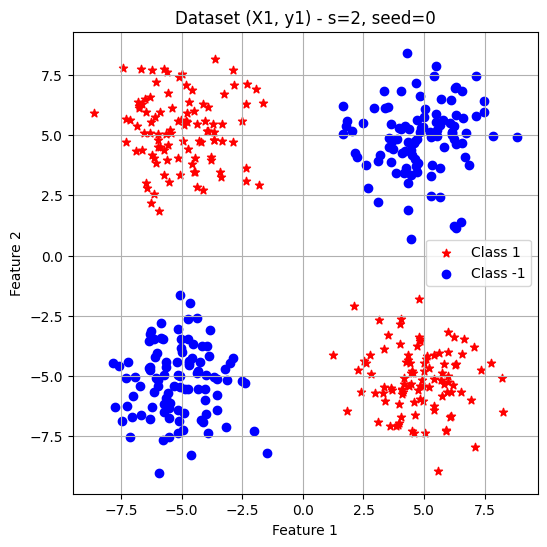
\includegraphics[width=\textwidth]{PR dataset.png}
        \caption{Dataset (X1, y1) - s=2, seed=0}
        \label{fig:dataset1}
    \end{subfigure}
    \hfill
    \begin{subfigure}{0.45\textwidth}
        \centering
        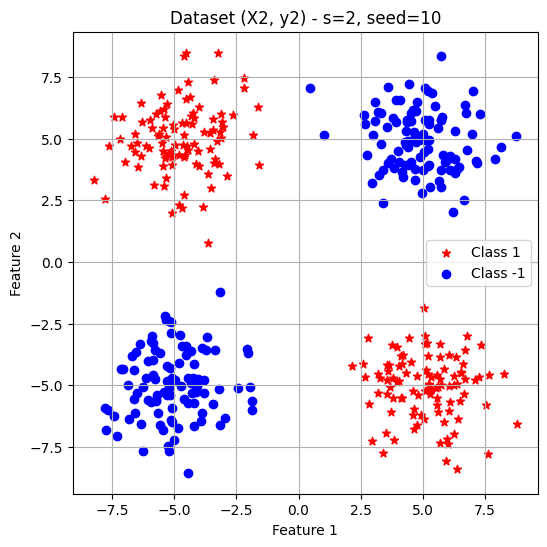
\includegraphics[width=\textwidth]{PR dataset2.png}
        \caption{Dataset (X2, y2) - s=2, seed=10}
        \label{fig:dataset2}
    \end{subfigure}
    
    \begin{subfigure}{0.45\textwidth}
        \centering
        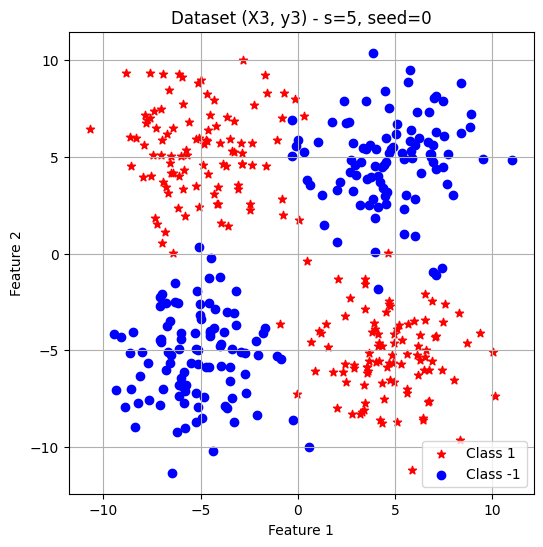
\includegraphics[width=\textwidth]{PR dataset3.png}
        \caption{Dataset (X3, y3) - s=5, seed=0}
        \label{fig:dataset3}
    \end{subfigure}
    \hfill
    \begin{subfigure}{0.45\textwidth}
        \centering
        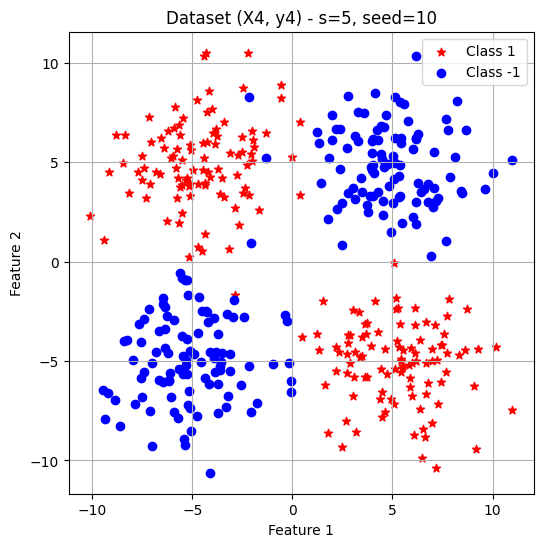
\includegraphics[width=\textwidth]{PR dataset4.png}
        \caption{Dataset (X4, y4) - s=5, seed=10}
        \label{fig:dataset4}
    \end{subfigure}

    \caption{Comparison of datasets generated with different seeds and variance values}
    \label{fig:all_datasets}
\end{figure}

\newpage


\subsection{Standard Backpropagation Algorithm}
\textbf{(a)} Run the standard backpropagation algorithm with $lr = 0.01$ and 2, 4, and 15 first-layer nodes, for 1000 iterations, using the dataset $(X_1, y_1)$ as the training set.
\\
\textbf{(b)} Evaluate the performance of the designed neural networks for both $(X_1, y_1)$ (training set) and $(X_2, y_2)$ (test set) and plot the decision regions (use $lb = lv = -10, ub = uv = 10, rb = rv = 0.2$).
\\ 
\textbf{(c)} Comment on the results. \\
\\
\textbf{Answer:} 

\begin{figure}[H]
    \centering
    \captionsetup[subfigure]{list=true} % Ensure subfigures appear in LoF

    \begin{subfigure}{0.5\textwidth}
        \centering
        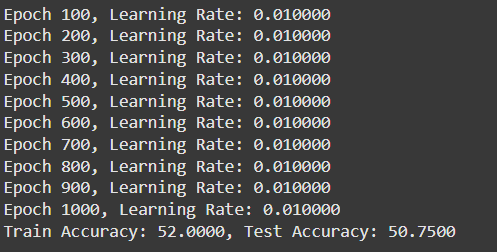
\includegraphics[width=\textwidth]{2.2_2_r.png}
        \caption{Result of 2 first layer nodes}
    \end{subfigure}
    \begin{subfigure}{0.45\textwidth}
        \centering
        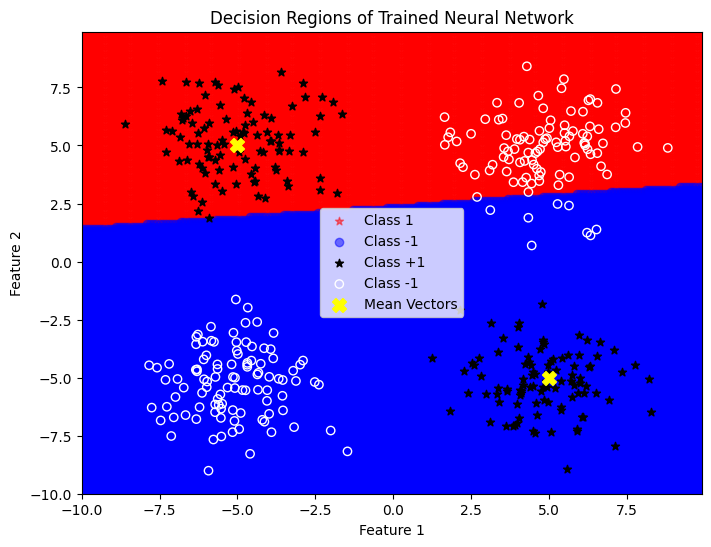
\includegraphics[width=\textwidth]{2.2_2_Train.png}
        \caption{Training set decision boundary}
    \end{subfigure}

    \begin{subfigure}{0.45\textwidth}
        \centering
        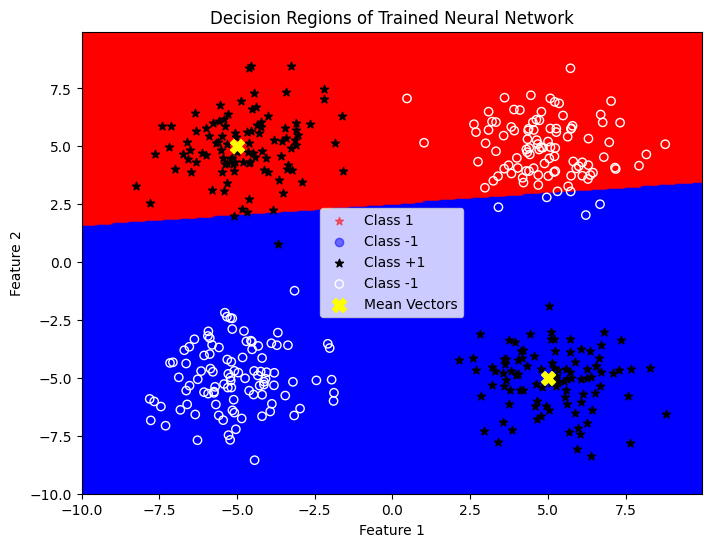
\includegraphics[width=\textwidth]{2.2_2_Test.png}
        \caption{Test set decision boundary}
    \end{subfigure}

    \caption{Comparison of decision regions and boundaries for training and test sets for 2 first layer nodes} 
\end{figure}

\begin{figure}[H]
    \centering
    \captionsetup[subfigure]{list=true} % Ensure subfigures appear in LoF

    \begin{subfigure}{0.5\textwidth}
        \centering
        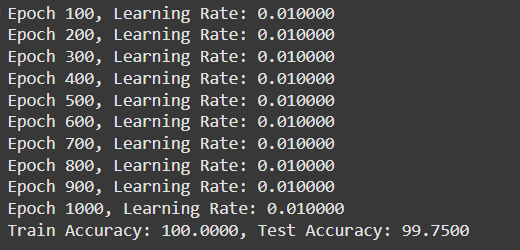
\includegraphics[width=\textwidth]{2.2_4_r.png}
        \caption{Result of 4 first layer nodes}
    \end{subfigure}
    \begin{subfigure}{0.45\textwidth}
        \centering
        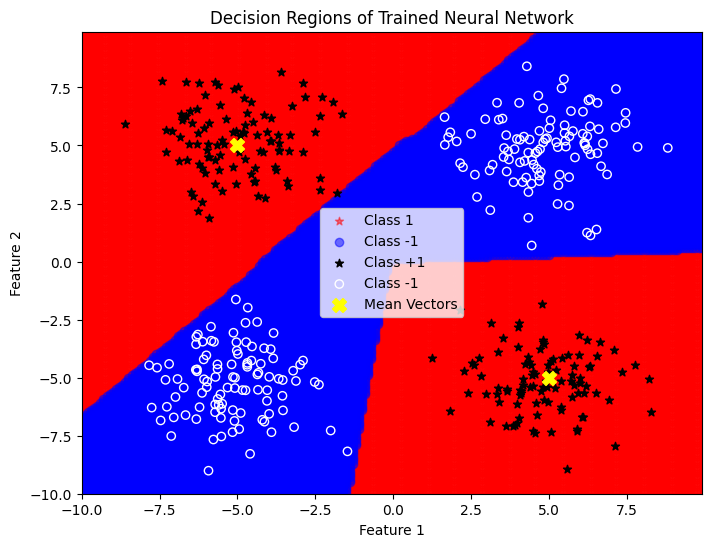
\includegraphics[width=\textwidth]{2.2_4_Train.png}
        \caption{Training set decision boundary}
    \end{subfigure}

    \begin{subfigure}{0.45\textwidth}
        \centering
        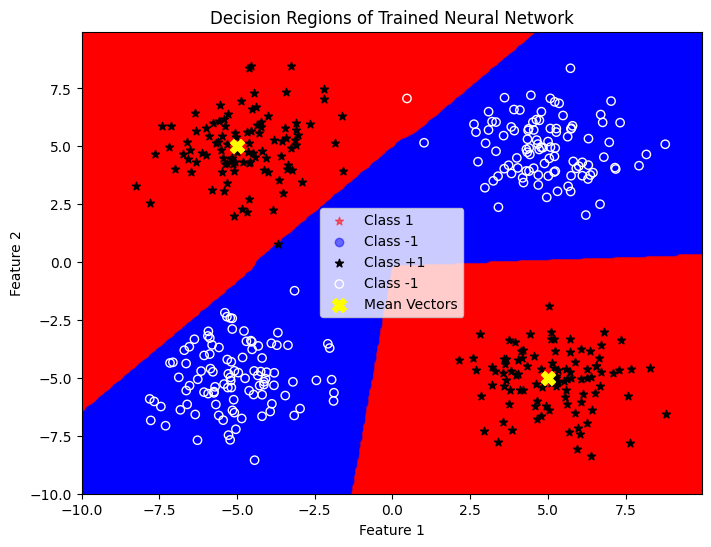
\includegraphics[width=\textwidth]{2.2_4_Test.png}
        \caption{Test set decision boundary}
    \end{subfigure}

    \caption{Comparison of decision regions and boundaries for training and test sets for 4 first layer nodes} 
\end{figure}

\begin{figure}[H]
    \centering
    \captionsetup[subfigure]{list=true} % Ensure subfigures appear in LoF

    \begin{subfigure}{0.5\textwidth}
        \centering
        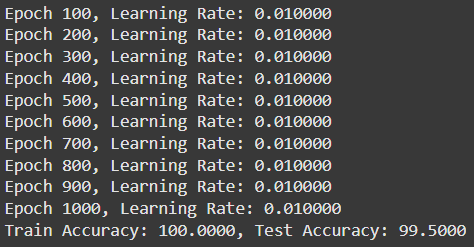
\includegraphics[width=\textwidth]{2.2_15_r.png}
        \caption{Result of 15 first layer nodes}
    \end{subfigure}
    \begin{subfigure}{0.45\textwidth}
        \centering
        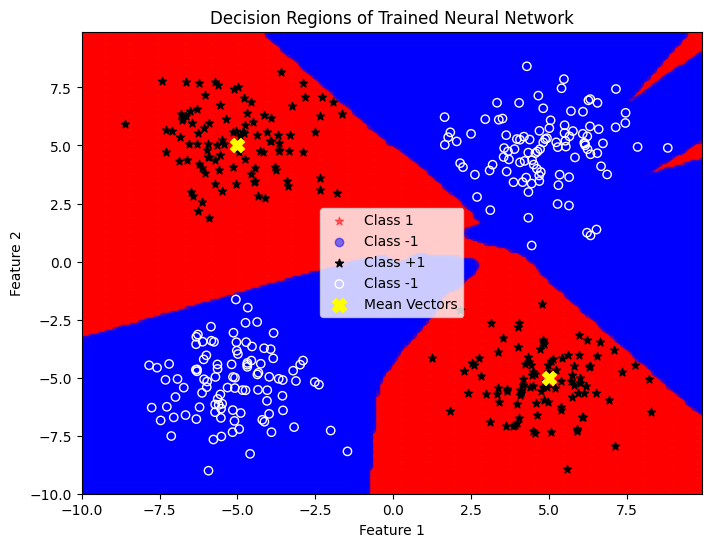
\includegraphics[width=\textwidth]{2.2_15_Train.png}
        \caption{Training set decision boundary}
    \end{subfigure}

    \begin{subfigure}{0.45\textwidth}
        \centering
        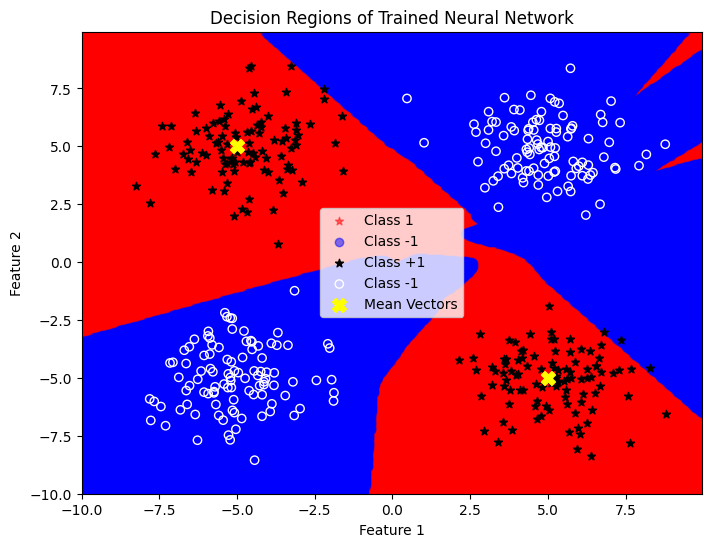
\includegraphics[width=\textwidth]{2.2_15_Test.png}
        \caption{Test set decision boundary}
    \end{subfigure}

    \caption{Comparison of decision regions and boundaries for training and test sets for 15 first layer nodes} 
\end{figure}
From the above figures, we can see that accuracy increases with the number of nodes in the first layer. The decision boundary becomes more complex and better fits the training data, but it also risks overfitting, especially with 15 nodes. The test set accuracy is lower than the training set accuracy, indicating some overfitting.
\newpage
\subsection{Backpropagation Algorithm with Different Learning Rates}
\textbf{(a)} Run the backpropagation algorithm with 4 first-layer nodes with the following settings:

\hspace{5mm} $-$ $lr = 0.01$, for 300 iterations.  

\hspace{5mm} $-$ $lr = 0.001$, for 300 iterations.  

\hspace{5mm} $-$ $lr = 0.01$, for 1000 iterations.  

\hspace{5mm} $-$ $lr = 0.001$, for 1000 iterations.  

Use the dataset $(X_1, y_1)$ as the training set.

\textbf{(b)} Evaluate the performance of the designed neural networks for both $(X_1, y_1)$ (training set) and $(X_2, y_2)$ (test set) and plot the decision regions.
\\
\textbf{(c)} Comment on the results.\\
\\
\textbf{Answer:}

\begin{figure}[H]
    \centering
    \captionsetup[subfigure]{list=true} % Ensure subfigures appear in LoF

    \begin{subfigure}{0.5\textwidth}
        \centering
        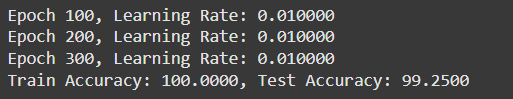
\includegraphics[width=\textwidth]{2.3_.01_300_r.png}
        \caption{lr = 0.01 for 300 iterations}
    \end{subfigure}
    \begin{subfigure}{0.45\textwidth}
        \centering
        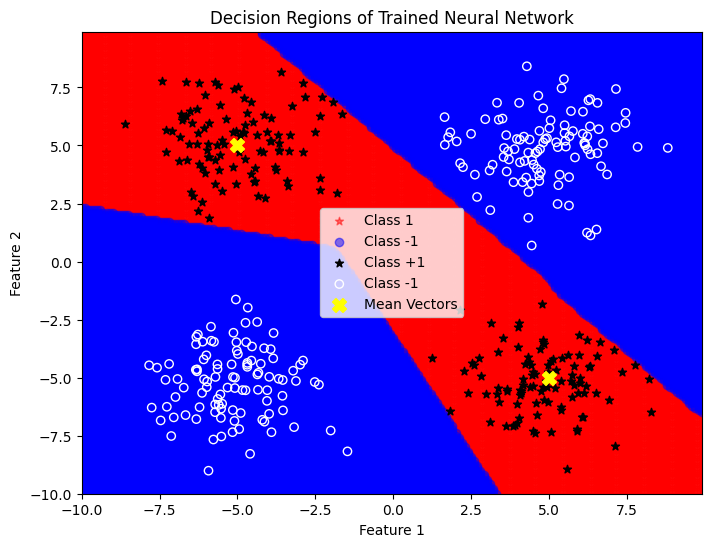
\includegraphics[width=\textwidth]{2.3_.01_300_Train.png}
        \caption{Training set decision boundary}
    \end{subfigure}

    \begin{subfigure}{0.45\textwidth}
        \centering
        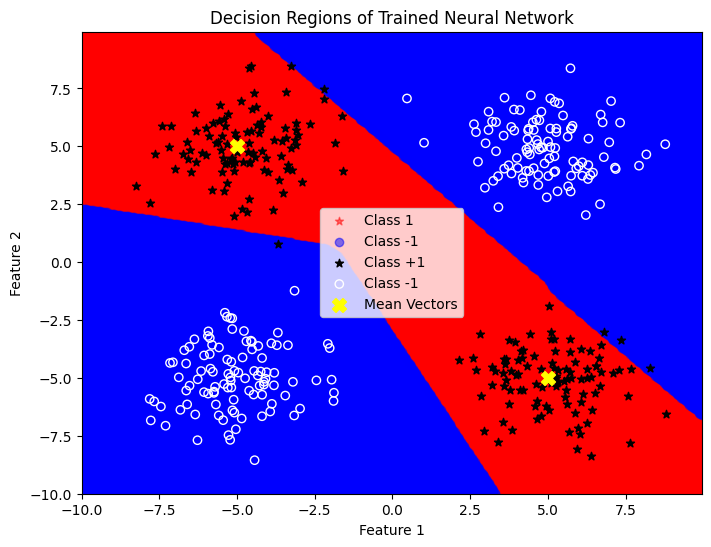
\includegraphics[width=\textwidth]{2.3_.01_300_Test.png}
        \caption{Test set decision boundary}
    \end{subfigure}

    \caption{Comparison of decision regions and boundaries for training and test sets for lr = 0.01 for 300 iterations}
\end{figure}

\begin{figure}[H]
    \centering
    \captionsetup[subfigure]{list=true} % Ensure subfigures appear in LoF

    \begin{subfigure}{0.5\textwidth}
        \centering
        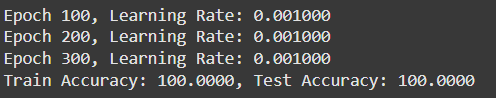
\includegraphics[width=\textwidth]{2.3_.001_300_r.png}
        \caption{lr = 0.001 for 300 iterations}
    \end{subfigure}
    \begin{subfigure}{0.45\textwidth}
        \centering
        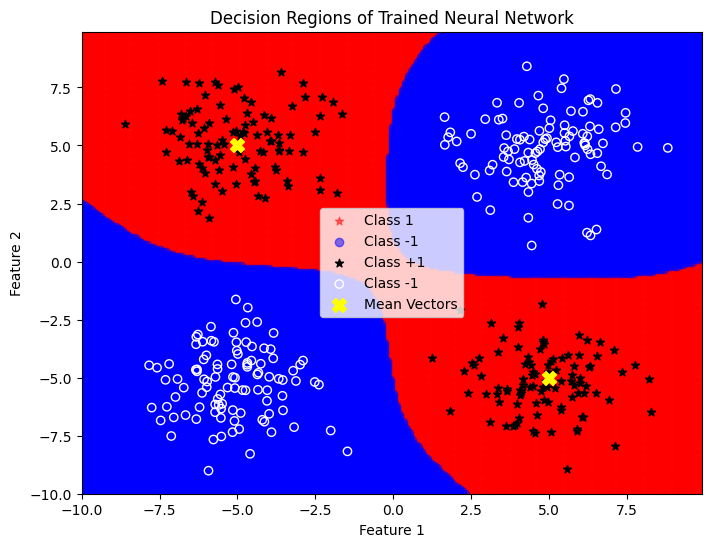
\includegraphics[width=\textwidth]{2.3_.001_300_Train.png}
        \caption{Training set decision boundary}
    \end{subfigure}

    \begin{subfigure}{0.45\textwidth}
        \centering
        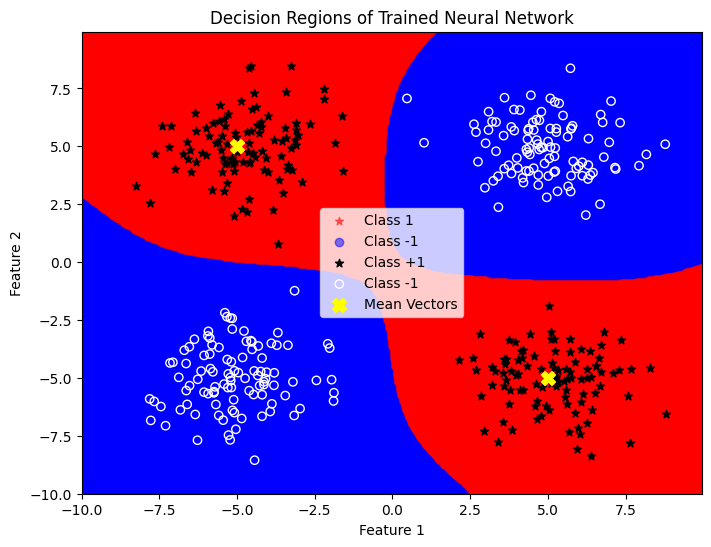
\includegraphics[width=\textwidth]{2.3_.001_300_Test.png}
        \caption{Test set decision boundary}
    \end{subfigure}

    \caption{Comparison of decision regions and boundaries for training and test sets for lr = 0.001 for 300 iterations}
\end{figure}

\begin{figure}[H]
    \centering
    \captionsetup[subfigure]{list=true} % Ensure subfigures appear in LoF

    \begin{subfigure}{0.5\textwidth}
        \centering
        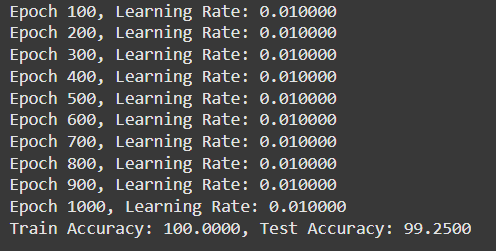
\includegraphics[width=\textwidth]{2.3_.01_1000_r.png}
        \caption{lr = 0.01 for 1000 iterations}
    \end{subfigure}
    \begin{subfigure}{0.45\textwidth}
        \centering
        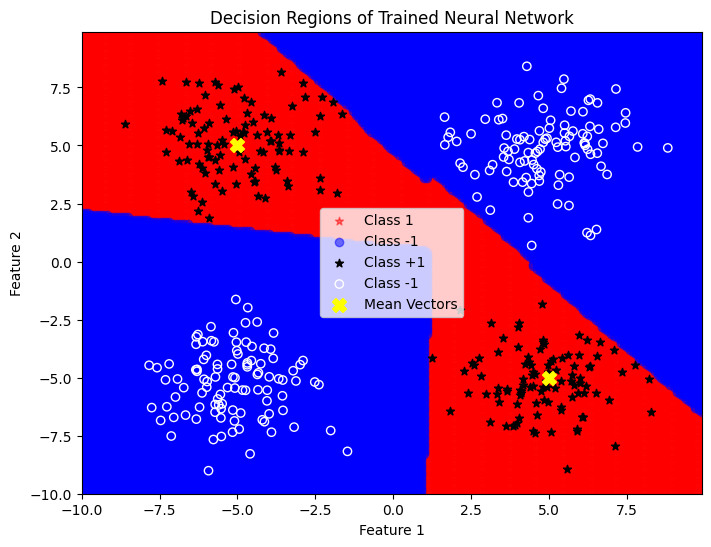
\includegraphics[width=\textwidth]{2.3_.01_1000_Train.png}
        \caption{Training set decision boundary}
    \end{subfigure}

    \begin{subfigure}{0.45\textwidth}
        \centering
        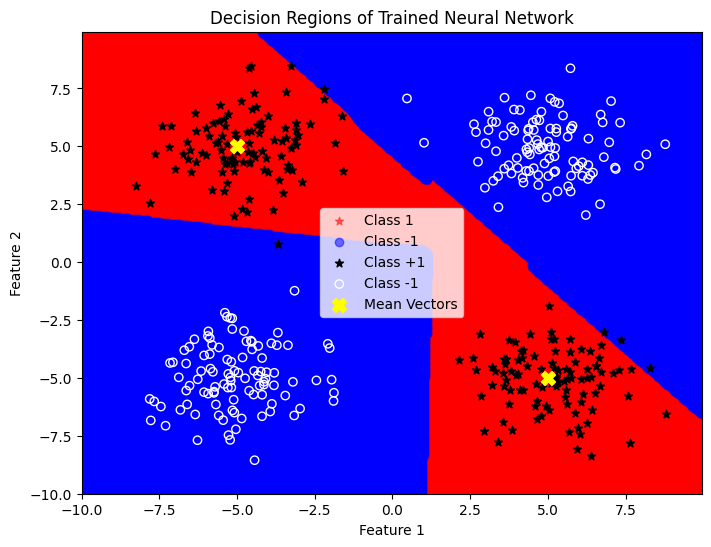
\includegraphics[width=\textwidth]{2.3_.01_1000_Test.png}
        \caption{Test set decision boundary}
    \end{subfigure}

    \caption{Comparison of decision regions and boundaries for training and test sets for lr = 0.01 for 1000 iterations}
\end{figure}

\begin{figure}[H]
    \centering
    \captionsetup[subfigure]{list=true} % Ensure subfigures appear in LoF

    \begin{subfigure}{0.5\textwidth}
        \centering
        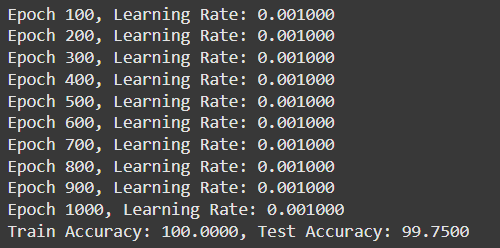
\includegraphics[width=\textwidth]{2.3_.001_1000_r.png}
        \caption{lr = 0.01 for 1000 iterations}
    \end{subfigure}
    \begin{subfigure}{0.45\textwidth}
        \centering
        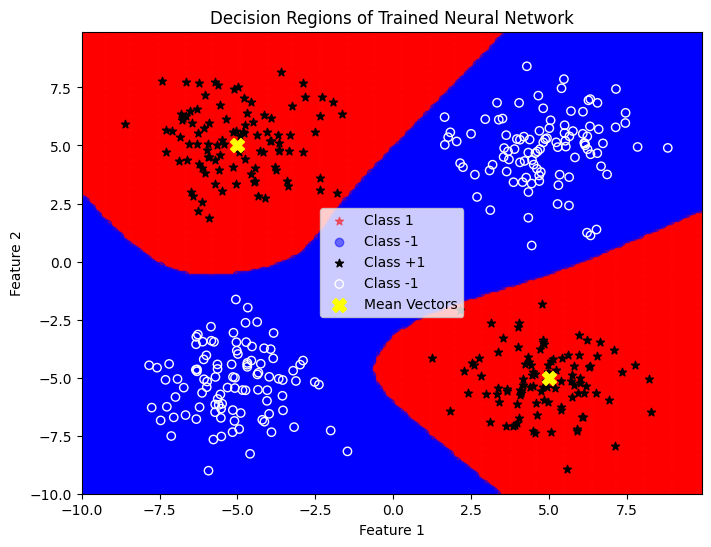
\includegraphics[width=\textwidth]{2.3_.001_1000_Train.png}
        \caption{Training set decision boundary}
    \end{subfigure}

    \begin{subfigure}{0.45\textwidth}
        \centering
        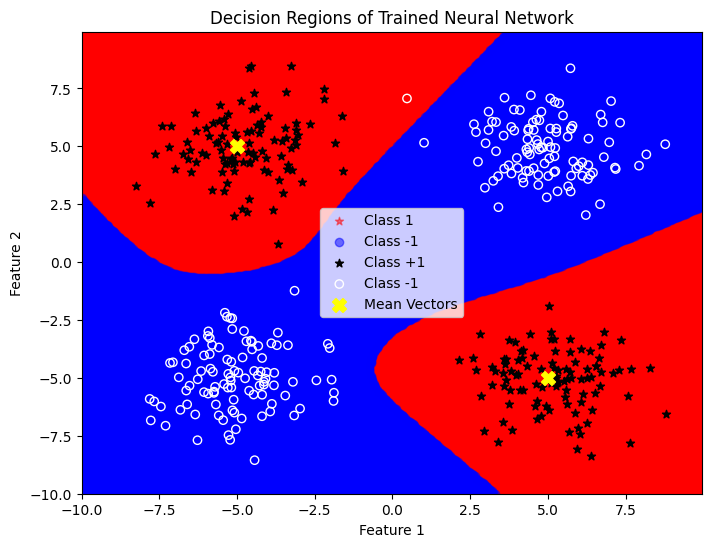
\includegraphics[width=\textwidth]{2.3_.001_1000_Test.png}
        \caption{Test set decision boundary}
    \end{subfigure}

    \caption{Comparison of decision regions and boundaries for training and test sets for lr = 0.001 for 1000 iterations}
\end{figure}

From the above figures, we can see that the learning rate significantly affects the convergence speed and the final decision boundary. A higher learning rate (0.01) converges faster but may overshoot the optimal solution, while a lower learning rate (0.001) converges more slowly but can lead to a more stable solution. The number of iterations also plays a crucial role; more iterations allow for better convergence, but they also increase the risk of overfitting, especially with a high learning rate.
\newpage
\subsection{Adaptive Learning Rate Backpropagation}
\textbf{(a)} Run the adaptive learning rate variation of the backpropagation algorithm with the following parameters:

\hspace{5mm} $-$ $lr = 0.001$  

\hspace{5mm} $-$ $lr_{inc} = 1.05$  

\hspace{5mm} $-$ $lr_{dec} = 0.7$  

\hspace{5mm} $-$ $max\_perf\_inc = 1.04$  

Run the algorithm for 300 iterations.

\textbf{(b)} Evaluate the performance of the designed neural networks for both $(X_1, y_1)$ (training set) and $(X_2, y_2)$ (test set) and plot the decision regions.
\textbf{(c)} Compare the above results with those obtained for the standard backpropagation algorithm with $lr = 0.001$, for 300 iterations.
\\
\textbf{Answer:}\\

\begin{figure}[H]
    \centering
    \captionsetup[subfigure]{list=true} % Ensure subfigures appear in LoF

    \begin{subfigure}{0.5\textwidth}
        \centering
        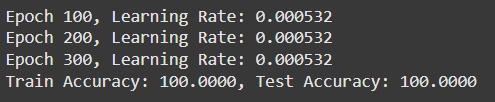
\includegraphics[width=\textwidth]{2.4_r.png}
        \caption{Result}
    \end{subfigure}
    \begin{subfigure}{0.45\textwidth}
        \centering
        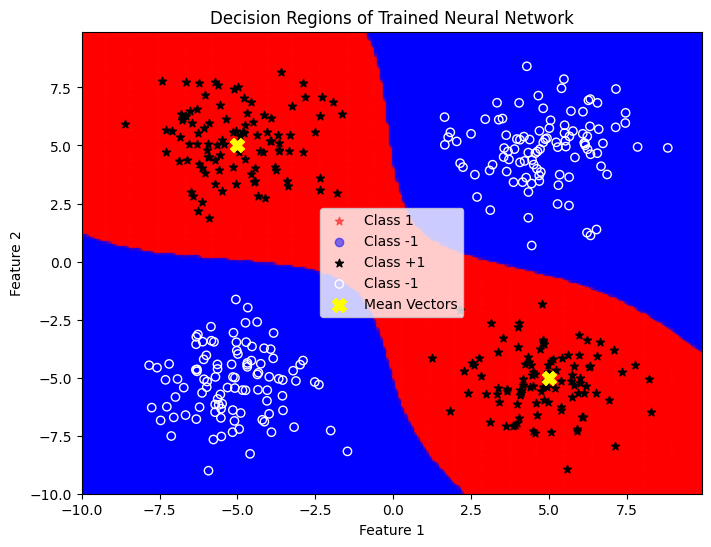
\includegraphics[width=\textwidth]{2.4_Train.png}
        \caption{Training set decision boundary}
    \end{subfigure}

    \begin{subfigure}{0.45\textwidth}
        \centering
        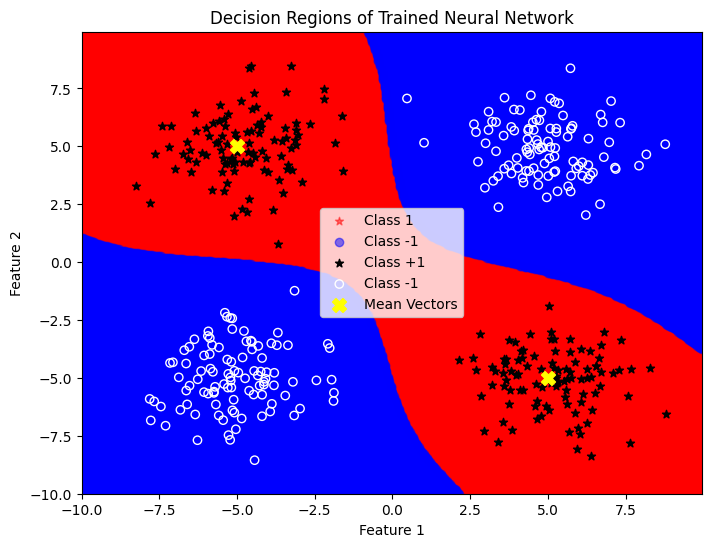
\includegraphics[width=\textwidth]{2.4_Test.png}
        \caption{Test set decision boundary}
    \end{subfigure}

        \caption{Comparison of decision regions and boundaries for training and test sets using adaptive learning rate backpropagation}
\end{figure}
The change in learning rate is not seen for lr= 0.001 but can be seen if its changed to 0.01 with more iterations. This is experimentally checked.
From the results, it is evident that the adaptive learning rate backpropagation algorithm performs better than the standard backpropagation algorithm with a fixed learning rate of 0.001 for 300 iterations. The adaptive learning rate allows the model to dynamically adjust the learning rate based on the performance, leading to faster convergence and a more accurate decision boundary. In contrast, the fixed learning rate may result in slower convergence and suboptimal performance. The decision regions produced by both more or less same as our data set is relatively simple.
\newpage
\subsection{Repeating Experiments on Different Data Sets}
\textbf{(a)} Repeat \textbf{Sections 2.2–2.4} using the datasets $(X_3, y_3)$ and $(X_4, y_4)$ as training and test sets, respectively.\\
\textbf{Answer:}
\begin{figure}[H]
    \centering
    \captionsetup[subfigure]{list=true} % Ensure subfigures appear in LoF

    \begin{subfigure}{0.5\textwidth}
        \centering
        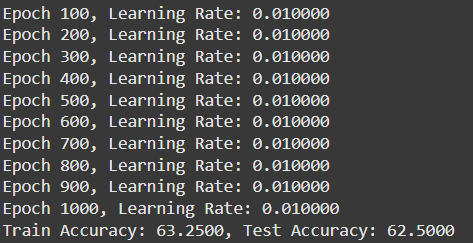
\includegraphics[width=\textwidth]{3.2_2_r.png}
        \caption{Result of 2 first layer nodes}
    \end{subfigure}
    \begin{subfigure}{0.45\textwidth}
        \centering
        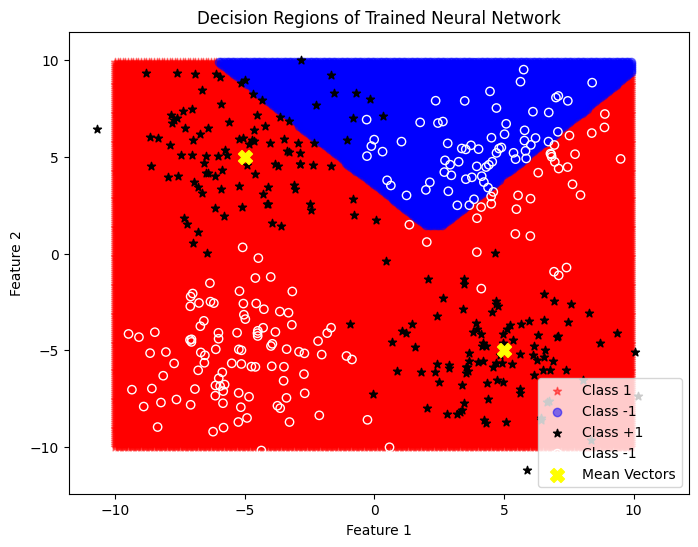
\includegraphics[width=\textwidth]{3.2_2_Train.png}
        \caption{Training set decision boundary}
    \end{subfigure}

    \begin{subfigure}{0.45\textwidth}
        \centering
        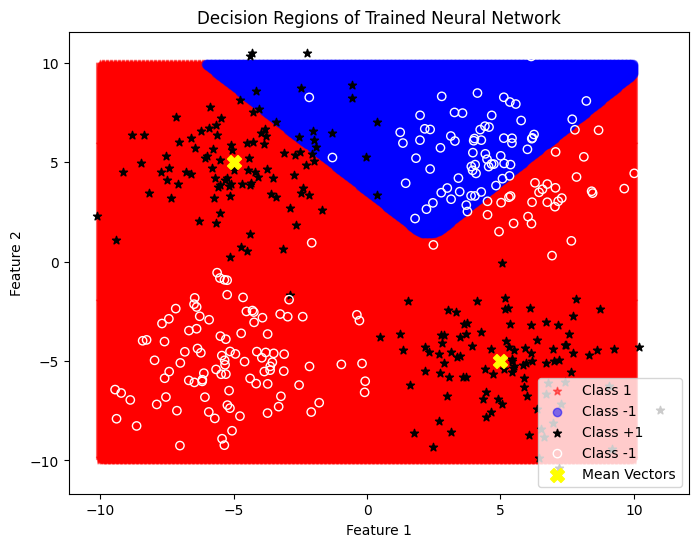
\includegraphics[width=\textwidth]{3.2_2_Test.png}
        \caption{Test set decision boundary}
    \end{subfigure}

    \caption{Comparison of decision regions and boundaries for training and test sets for 2 first layer nodes} 
\end{figure}

\begin{figure}[H]
    \centering
    \captionsetup[subfigure]{list=true} % Ensure subfigures appear in LoF

    \begin{subfigure}{0.5\textwidth}
        \centering
        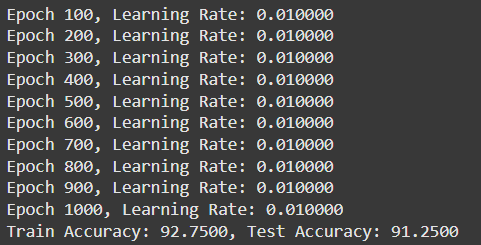
\includegraphics[width=\textwidth]{3.2_4_r.png}
        \caption{Result of 4 first layer nodes}
    \end{subfigure}
    \begin{subfigure}{0.45\textwidth}
        \centering
        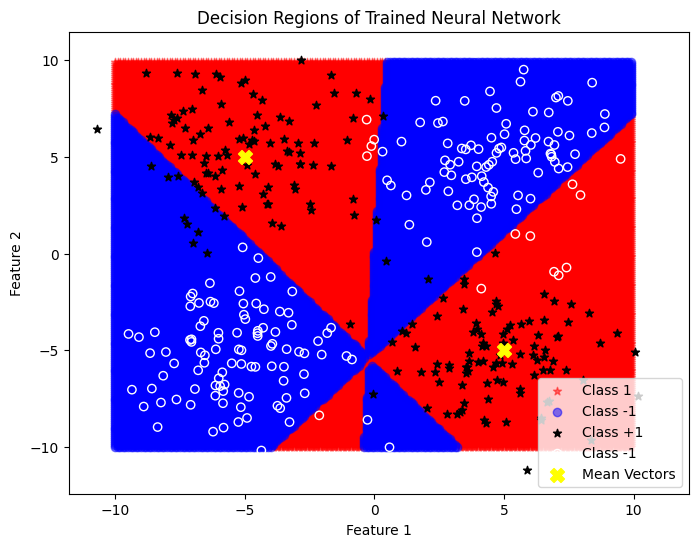
\includegraphics[width=\textwidth]{3.2_4_Train.png}
        \caption{Training set decision boundary}
    \end{subfigure}

    \begin{subfigure}{0.45\textwidth}
        \centering
        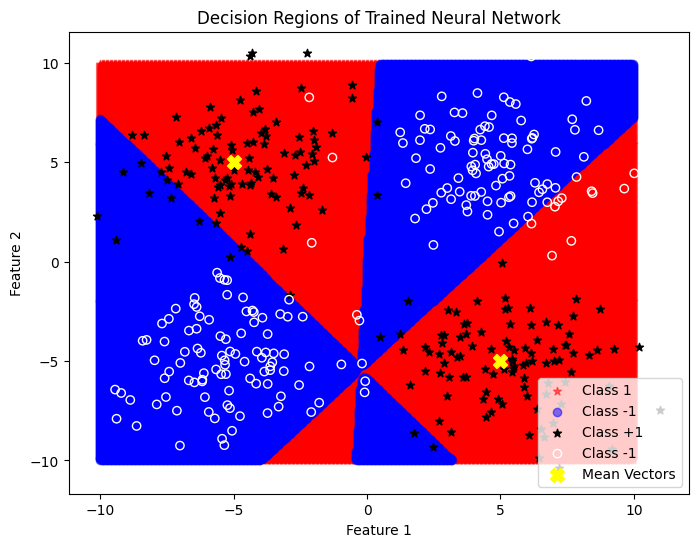
\includegraphics[width=\textwidth]{3.2_4_Test.png}
        \caption{Test set decision boundary}
    \end{subfigure}

    \caption{Comparison of decision regions and boundaries for training and test sets for 4 first layer nodes} 
\end{figure}

\begin{figure}[H]
    \centering
    \captionsetup[subfigure]{list=true} % Ensure subfigures appear in LoF

    \begin{subfigure}{0.5\textwidth}
        \centering
        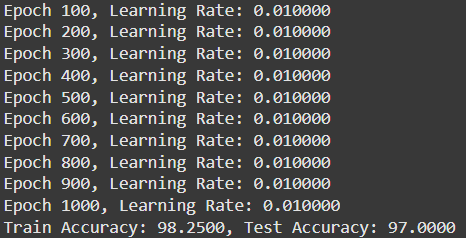
\includegraphics[width=\textwidth]{3.2_15_r.png}
        \caption{Result of 15 first layer nodes}
    \end{subfigure}
    \begin{subfigure}{0.45\textwidth}
        \centering
        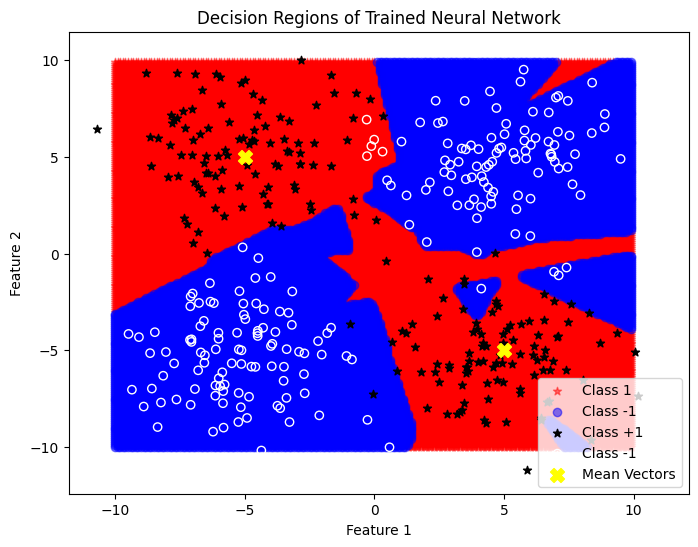
\includegraphics[width=\textwidth]{3.2_15_Train.png}
        \caption{Training set decision boundary}
    \end{subfigure}

    \begin{subfigure}{0.45\textwidth}
        \centering
        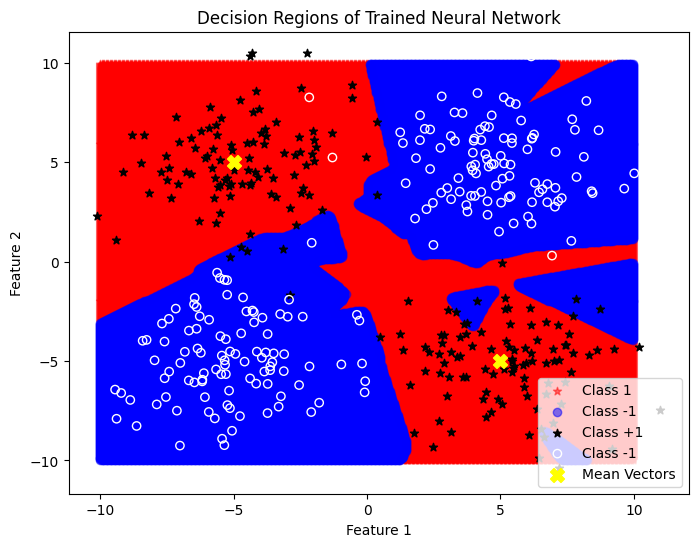
\includegraphics[width=\textwidth]{3.2_15_Test.png}
        \caption{Test set decision boundary}
    \end{subfigure}

    \caption{Comparison of decision regions and boundaries for training and test sets for 15 first layer nodes} 
\end{figure}

\begin{figure}[H]
    \centering
    \captionsetup[subfigure]{list=true} % Ensure subfigures appear in LoF

    \begin{subfigure}{0.5\textwidth}
        \centering
        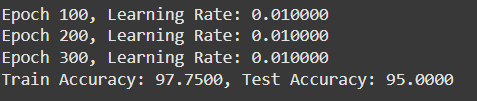
\includegraphics[width=\textwidth]{3.3_.01_300_r.png}
        \caption{lr = 0.01 for 300 iterations}
    \end{subfigure}
    \begin{subfigure}{0.45\textwidth}
        \centering
        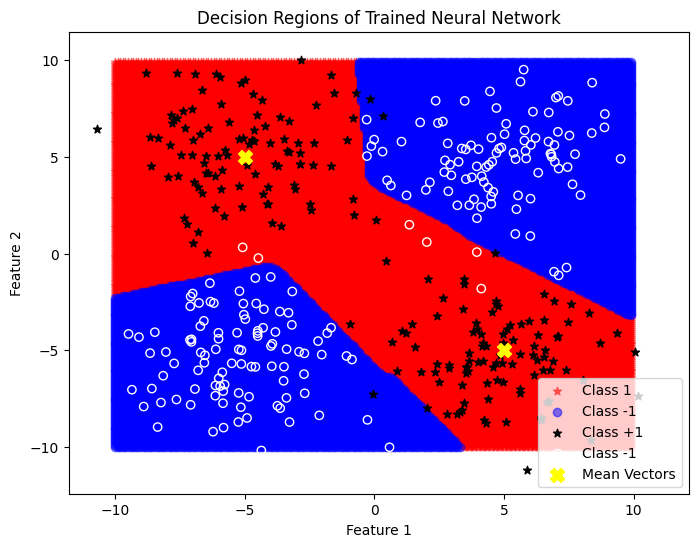
\includegraphics[width=\textwidth]{3.3_.01_300_Train.png}
        \caption{Training set decision boundary}
    \end{subfigure}

    \begin{subfigure}{0.45\textwidth}
        \centering
        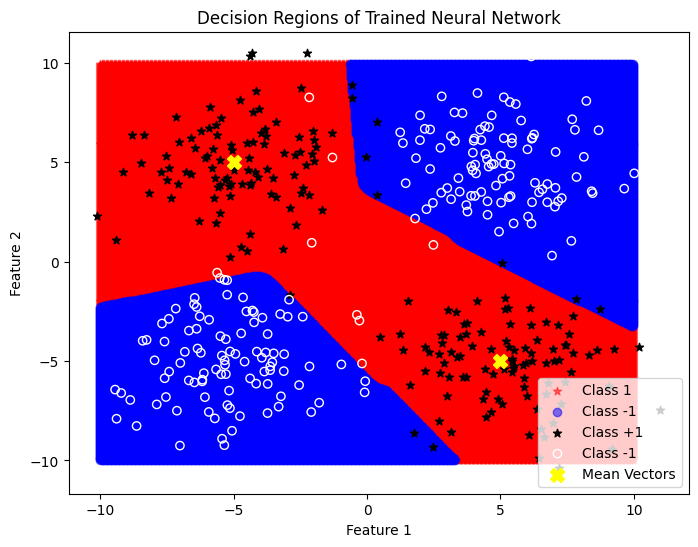
\includegraphics[width=\textwidth]{3.3_.01_300_Test.png}
        \caption{Test set decision boundary}
    \end{subfigure}

    \caption{Comparison of decision regions and boundaries for training and test sets for lr = 0.01 for 300 iterations}
\end{figure}

\begin{figure}[H]
    \centering
    \captionsetup[subfigure]{list=true} % Ensure subfigures appear in LoF

    \begin{subfigure}{0.5\textwidth}
        \centering
        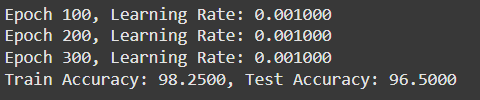
\includegraphics[width=\textwidth]{3.3_.001_300_r.png}
        \caption{lr = 0.001 for 300 iterations}
    \end{subfigure}
    \begin{subfigure}{0.45\textwidth}
        \centering
        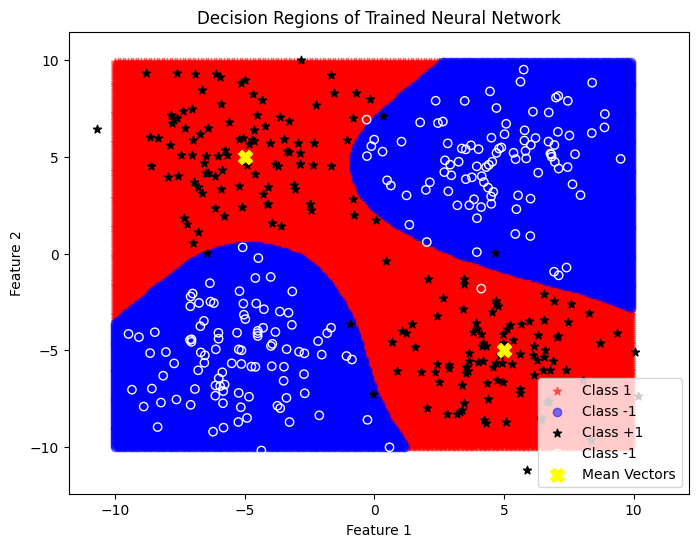
\includegraphics[width=\textwidth]{3.3_.001_300_Train.png}
        \caption{Training set decision boundary}
    \end{subfigure}

    \begin{subfigure}{0.45\textwidth}
        \centering
        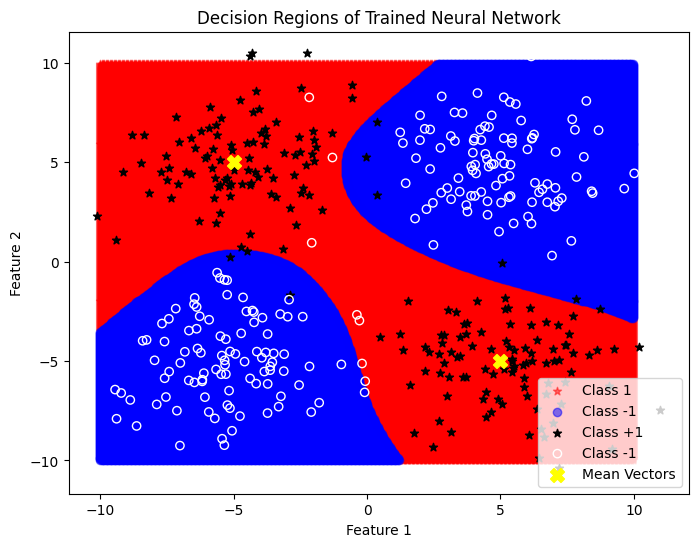
\includegraphics[width=\textwidth]{3.3_.001_300_Test.png}
        \caption{Test set decision boundary}
    \end{subfigure}

    \caption{Comparison of decision regions and boundaries for training and test sets for lr = 0.001 for 300 iterations}
\end{figure}

\begin{figure}[H]
    \centering
    \captionsetup[subfigure]{list=true} % Ensure subfigures appear in LoF

    \begin{subfigure}{0.5\textwidth}
        \centering
        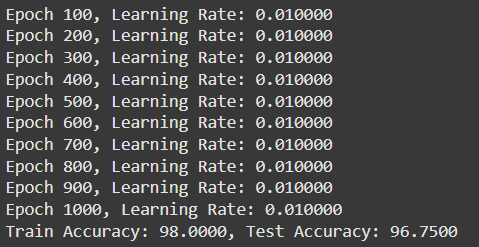
\includegraphics[width=\textwidth]{3.3_.01_1000_r.png}
        \caption{lr = 0.01 for 1000 iterations}
    \end{subfigure}
    \begin{subfigure}{0.45\textwidth}
        \centering
        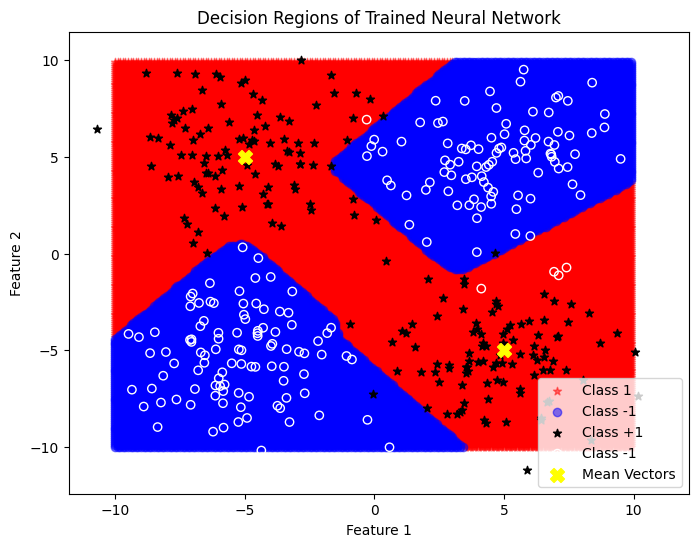
\includegraphics[width=\textwidth]{3.3_.01_1000_Train.png}
        \caption{Training set decision boundary}
    \end{subfigure}

    \begin{subfigure}{0.45\textwidth}
        \centering
        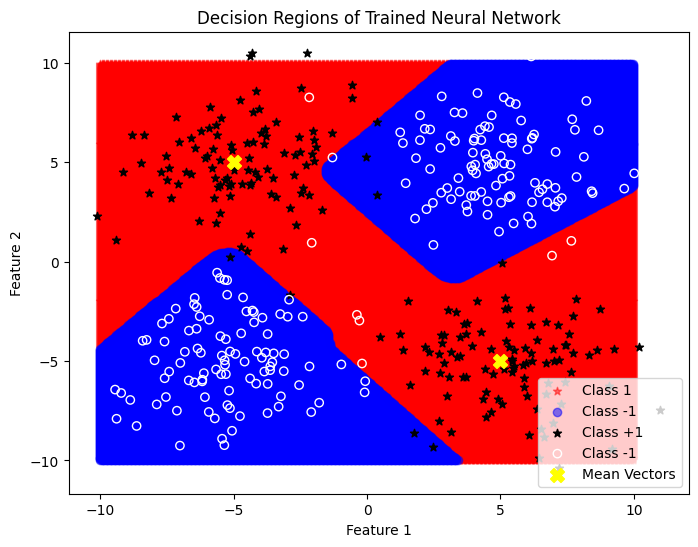
\includegraphics[width=\textwidth]{3.3_.01_1000_Test.png}
        \caption{Test set decision boundary}
    \end{subfigure}

    \caption{Comparison of decision regions and boundaries for training and test sets for lr = 0.01 for 1000 iterations}
\end{figure}

\begin{figure}[H]
    \centering
    \captionsetup[subfigure]{list=true} % Ensure subfigures appear in LoF

    \begin{subfigure}{0.5\textwidth}
        \centering
        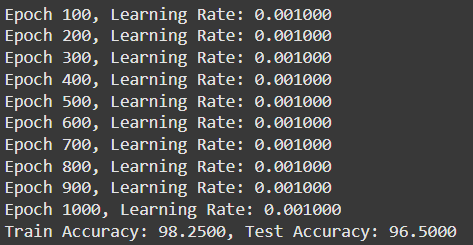
\includegraphics[width=\textwidth]{3.3_.001_1000_r.png}
        \caption{lr = 0.01 for 1000 iterations}
    \end{subfigure}
    \begin{subfigure}{0.45\textwidth}
        \centering
        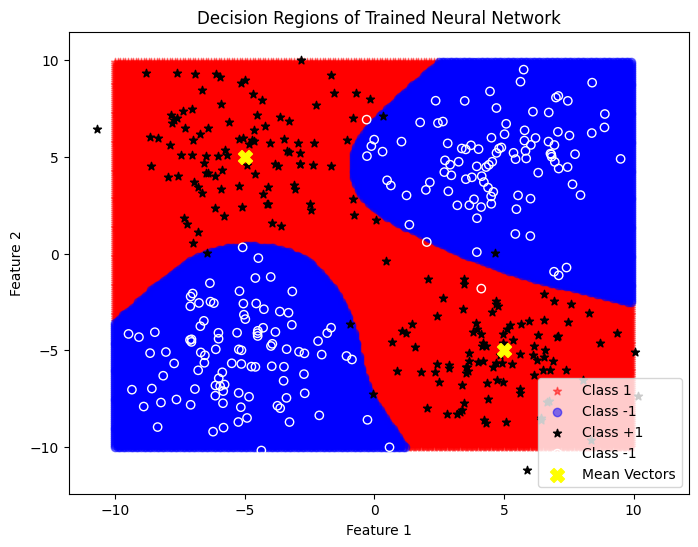
\includegraphics[width=\textwidth]{3.3_.001_1000_Train.png}
        \caption{Training set decision boundary}
    \end{subfigure}

    \begin{subfigure}{0.45\textwidth}
        \centering
        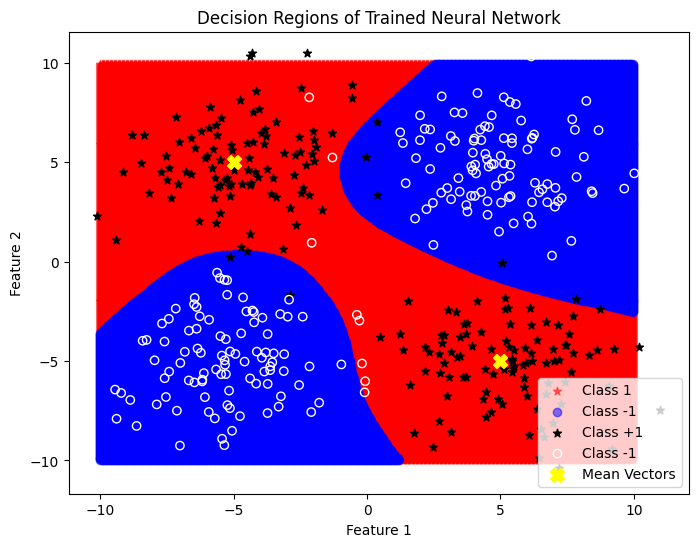
\includegraphics[width=\textwidth]{3.3_.001_1000_Test.png}
        \caption{Test set decision boundary}
    \end{subfigure}

    \caption{Comparison of decision regions and boundaries for training and test sets for lr = 0.001 for 1000 iterations}
\end{figure}

\begin{figure}[H]
    \centering
    \captionsetup[subfigure]{list=true} % Ensure subfigures appear in LoF

    \begin{subfigure}{0.5\textwidth}
        \centering
        \includegraphics[width=\textwidth]{3.4_r.png}
        \caption{Result}
    \end{subfigure}
    \begin{subfigure}{0.45\textwidth}
        \centering
        \includegraphics[width=\textwidth]{3.4_Train.png}
        \caption{Training set decision boundary}
    \end{subfigure}

    \begin{subfigure}{0.45\textwidth}
        \centering
        \includegraphics[width=\textwidth]{3.4_Test.png}
        \caption{Test set decision boundary}
    \end{subfigure}

        \caption{Comparison of decision regions and boundaries for training and test sets using adaptive learning rate backpropagation}
\end{figure}

 From above results we see that while repeating the same set of experiments with data set with little high variance the model accuracy is less  
 and decision boundaries are less sharp. This is expected as the data points are more spread out, making it harder 
 for the model to learn clear decision boundaries. Increasing the number of iterations or using more complex models might improve the performance.

\end{document}
